\documentclass[UKenglish]{beamer}

\usepackage[T1]{fontenc}

\usepackage{graphicx}

\usepackage[normalem]{ulem}

\usepackage{newclude}

% Haskell
\usepackage[cache=false]{minted}

\usepackage{tikz}
% Overlay effec
\usetikzlibrary{shapes.geometric,positioning,shapes.symbols,overlay-beamer-styles}

%% UIB
\usepackage[utf8]{inputenx} % For æ, ø, å
\usepackage{csquotes}       % Quotation marks
\usepackage{microtype}      % Improved typography
\usepackage{amssymb}        % Mathematical symbols
\usepackage{mathtools}      % Mathematical symbols
\usepackage[absolute, overlay]{textpos} % Arbitrary placement
\setlength{\TPHorizModule}{\paperwidth} % Textpos units
\setlength{\TPVertModule}{\paperheight} % Textpos units
%%

\title{Modular IDE Development Plan H24}
\author{Nils Michael Fitjar}
\date{\today}

\begin{document}

\frame{\titlepage}

\section{Plan}
\begin{frame}{Plan}
    \begin{itemize}
        \item \sout{Create an IDE}
        \item Create Plugins
        \item ...
        \item Profit
    \end{itemize}
\end{frame}

\section{Showcase}
\begin{frame}{IDE}
  So, here is my IDE:
\end{frame}

\begin{frame}{IDE Features}
  \begin{itemize}
    \item Dynamically loading of Plugins
  \end{itemize}
\end{frame}

\section{Plugins}
\begin{frame}{Loading of Plugins}
  A Plugin, is a C-library, that is dynamically loaded
  during startup.
  It needs to expose, an init, view and update function.
\end{frame}

\begin{frame}{Plugin Example}
  \begin{minted}{haskell}
-- Manifest :: Map
init :: Map
init :: [("counter", ValInt 0)]

update :: Msg -> Map -> Map
update (PluginMsg "counter") model =
  case lookup "counter" model of
    Just (ValInt i) -> insert "counter" (ValInt (i + 1)) model
    Nothing -> insert "counter" (ValInt 0) model

view :: Map -> Html
view model = Div [] [Text "Hello, World!"
  , Btn [OnClick (PluginMsg "counter")] []
  , Text (putStrLn (lookupOrDefault "counter" model))
\end{minted}



\end{frame}

\begin{frame}{Plugin Architecture}
    \begin{figure}
        \centering
        \begin{minted}{haskell}
-- Manifest :: Map
init :: Map
init :: [("counter", ValInt 0)]

update :: Msg -> Map -> Map
update (PluginMsg "counter") model =
  case lookup "counter" model of
    Just (ValInt i) -> insert "counter" (ValInt (i + 1)) model
    Nothing -> insert "counter" (ValInt 0) model

view :: Map -> Html
view model = Div [] [Text "Hello, World!"
  , Btn [OnClick (PluginMsg "counter")] []
  , Text (putStrLn (lookupOrDefault "counter" model))
\end{minted}



        \caption{Plugin Architecture}
    \end{figure}
\end{frame}

\section{Remaining Work}
\begin{frame}{Remaining Work}
\begin{itemize}
  \item Plugins
  \begin{itemize}
    \item Make useful plugins
      \begin{itemize}
        \item Plugin Mangers
      \end{itemize}
    \item Expand Plugin Language Landscape
      \begin{itemize}
        \item C
        \item Haskell
      \end{itemize}
  \end{itemize}

  \item Tests
  \begin{itemize}
    \item Unit Tests
    \item Memory Leak Tests
    \item Integration Tests
    \item Platform Tests
  \end{itemize}
  \item Building
  \begin{itemize}
    \item Figure out all necessary dependencies
    \item Ensure users can build for \textit{all} platforms
    \item Create installer?
  \end{itemize}
\end{itemize}
\end{frame}

\section{Plugin Manager}
\begin{frame}{Plugin Manager}
    \begin{figure}
        \centering
        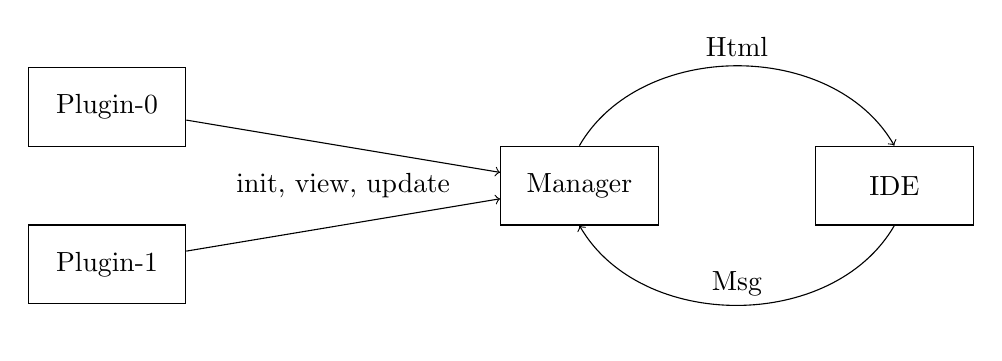
\begin{tikzpicture}
  % Nodes
  \node (p-0) [rectangle, draw, minimum height=1cm, minimum width=2cm] at (-5, 1) {Plugin-0};
  \node (p-1) [rectangle, draw, minimum height=1cm, minimum width=2cm] at (-5, -1) {Plugin-1};
  \node (m) [rectangle, draw, minimum height=1cm, minimum width=2cm] at (1, 0) {Manager};
  \node (i) [rectangle, draw, minimum height=1cm, minimum width=2cm] at (5, 0) {IDE};
  % Arrow
  \draw[->] (m.north) to[out=60, in=120] node[midway, above] {Html} (i.north);
  \draw[->] (i.south) to[out=-120, in=-60] node[midway, above] {Msg} (m.south);
  \draw[->] (p-0) -- (m) node[midway, above] {};
  \draw[->] (p-1) -- (m) node[midway, above] {};
  % Header
  \node (txt) at (-2, 0) {init, view, update};
\end{tikzpicture}


        \caption{Plugin-Manager Architecture}
    \end{figure}
\end{frame}

\begin{frame}{Plugin Manager}
\begin{itemize}
  \item Ensure no collision, Msg, Model
  \item Ensure no redundant update call
  \item Plugins can have a \textit{Manifest}(extra model)
    so to specify extra information, like what
    functions they have
  \item Can use this to create \textit{Framework}
    plugins, for Html-structure, styling, etc.
\end{itemize}
\end{frame}


\section{Main Content}
\begin{frame}{Profit}
    \begin{figure}
        \centering
        
\includegraphics[width=0.6\textwidth]{../../pics/grindset.png}
        \caption{Businessman}
    \end{figure}
\end{frame}
\end{document}
